\begin{frame}{GNU/Linux prima delle distribuzioni}
    \begin{itemize}
        \item Lorem ipsum dolor sit amet, consectetur adipiscing elit
        \item Aliquam blandit faucibus nisi, sit amet dapibus enim tempus eu
        \item Nulla commodo, erat quis gravida posuere, elit lacus lobortis est, quis porttitor odio mauris at libero
        \item Nam cursus est eget velit posuere pellentesque
        \item Vestibulum faucibus velit a augue condimentum quis convallis nulla gravida
    \end{itemize}
\end{frame}

%------------------------------------------------

\begin{frame}{Le prime distribuzioni GNU/Linux}
    \begin{itemize}
        \item Boot-root - 1992
        \item MCC Interim Linux - 1992
        \item Slackware - 1993
        \item Yggdrasil Linux (Plug-and-Play) - 1993
    \end{itemize}
\end{frame}

\begin{frame}{Boot-root}
    \centering
    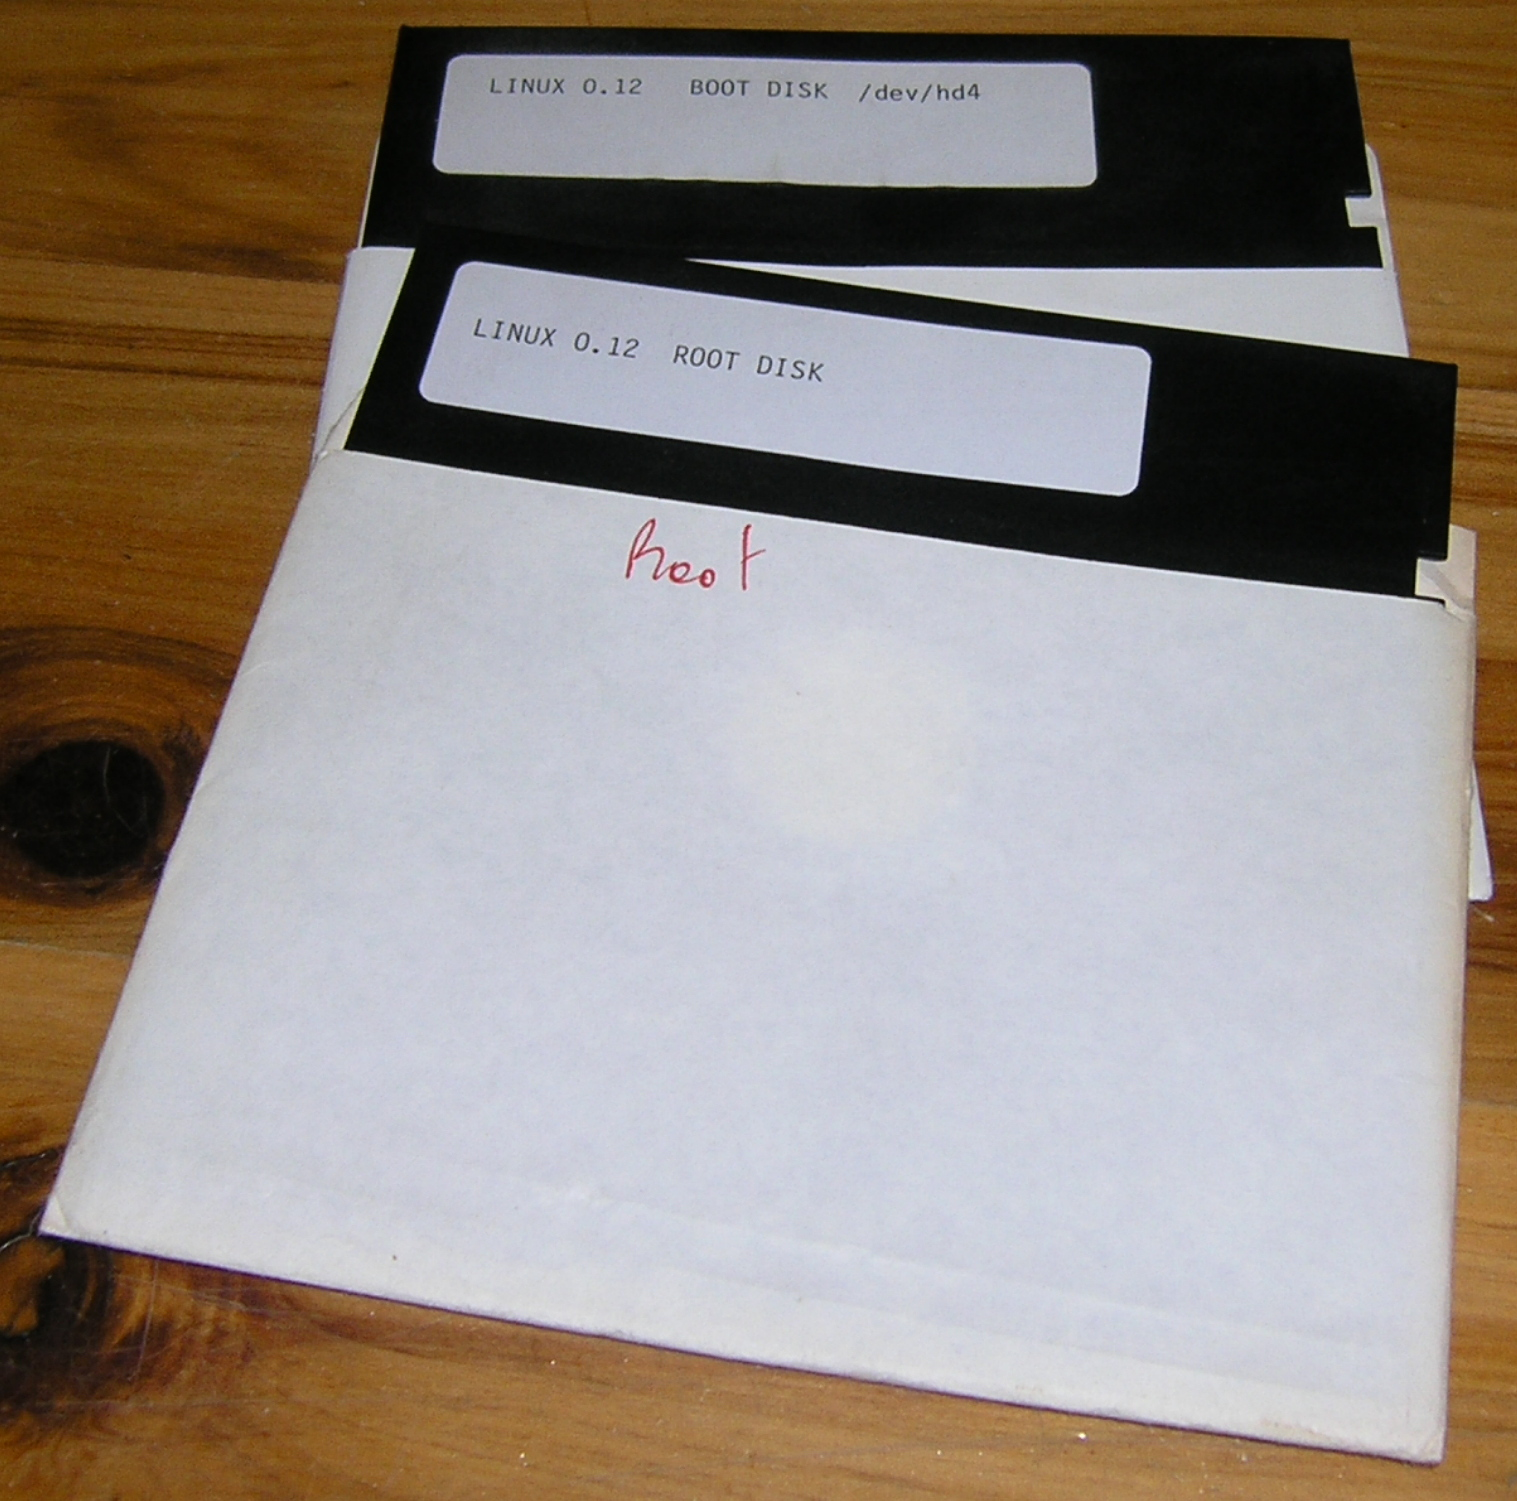
\includegraphics[scale=0.14]{images/Linux_0_12.jpg}
\end{frame}

%------------------------------------------------

\begin{frame}{Le distribuzioni GNU/Linux oggi}
    \centering
    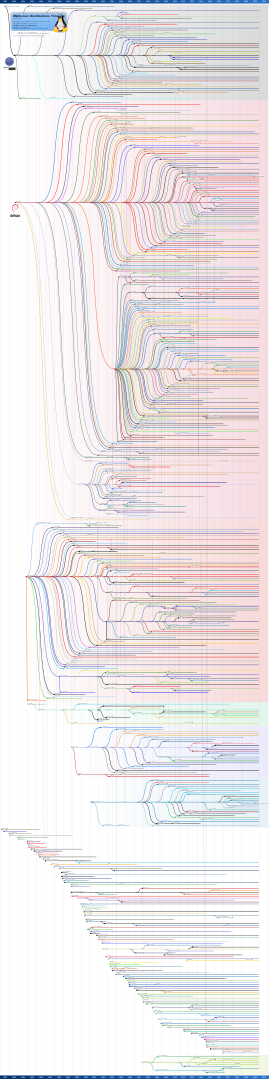
\includegraphics[scale=0.2]{images/Linux_Distribution_Timeline_Dec._2020.svg.png}
\end{frame}

\begin{frame}{Le distribuzioni GNU/Linux oggi}
    \centering
    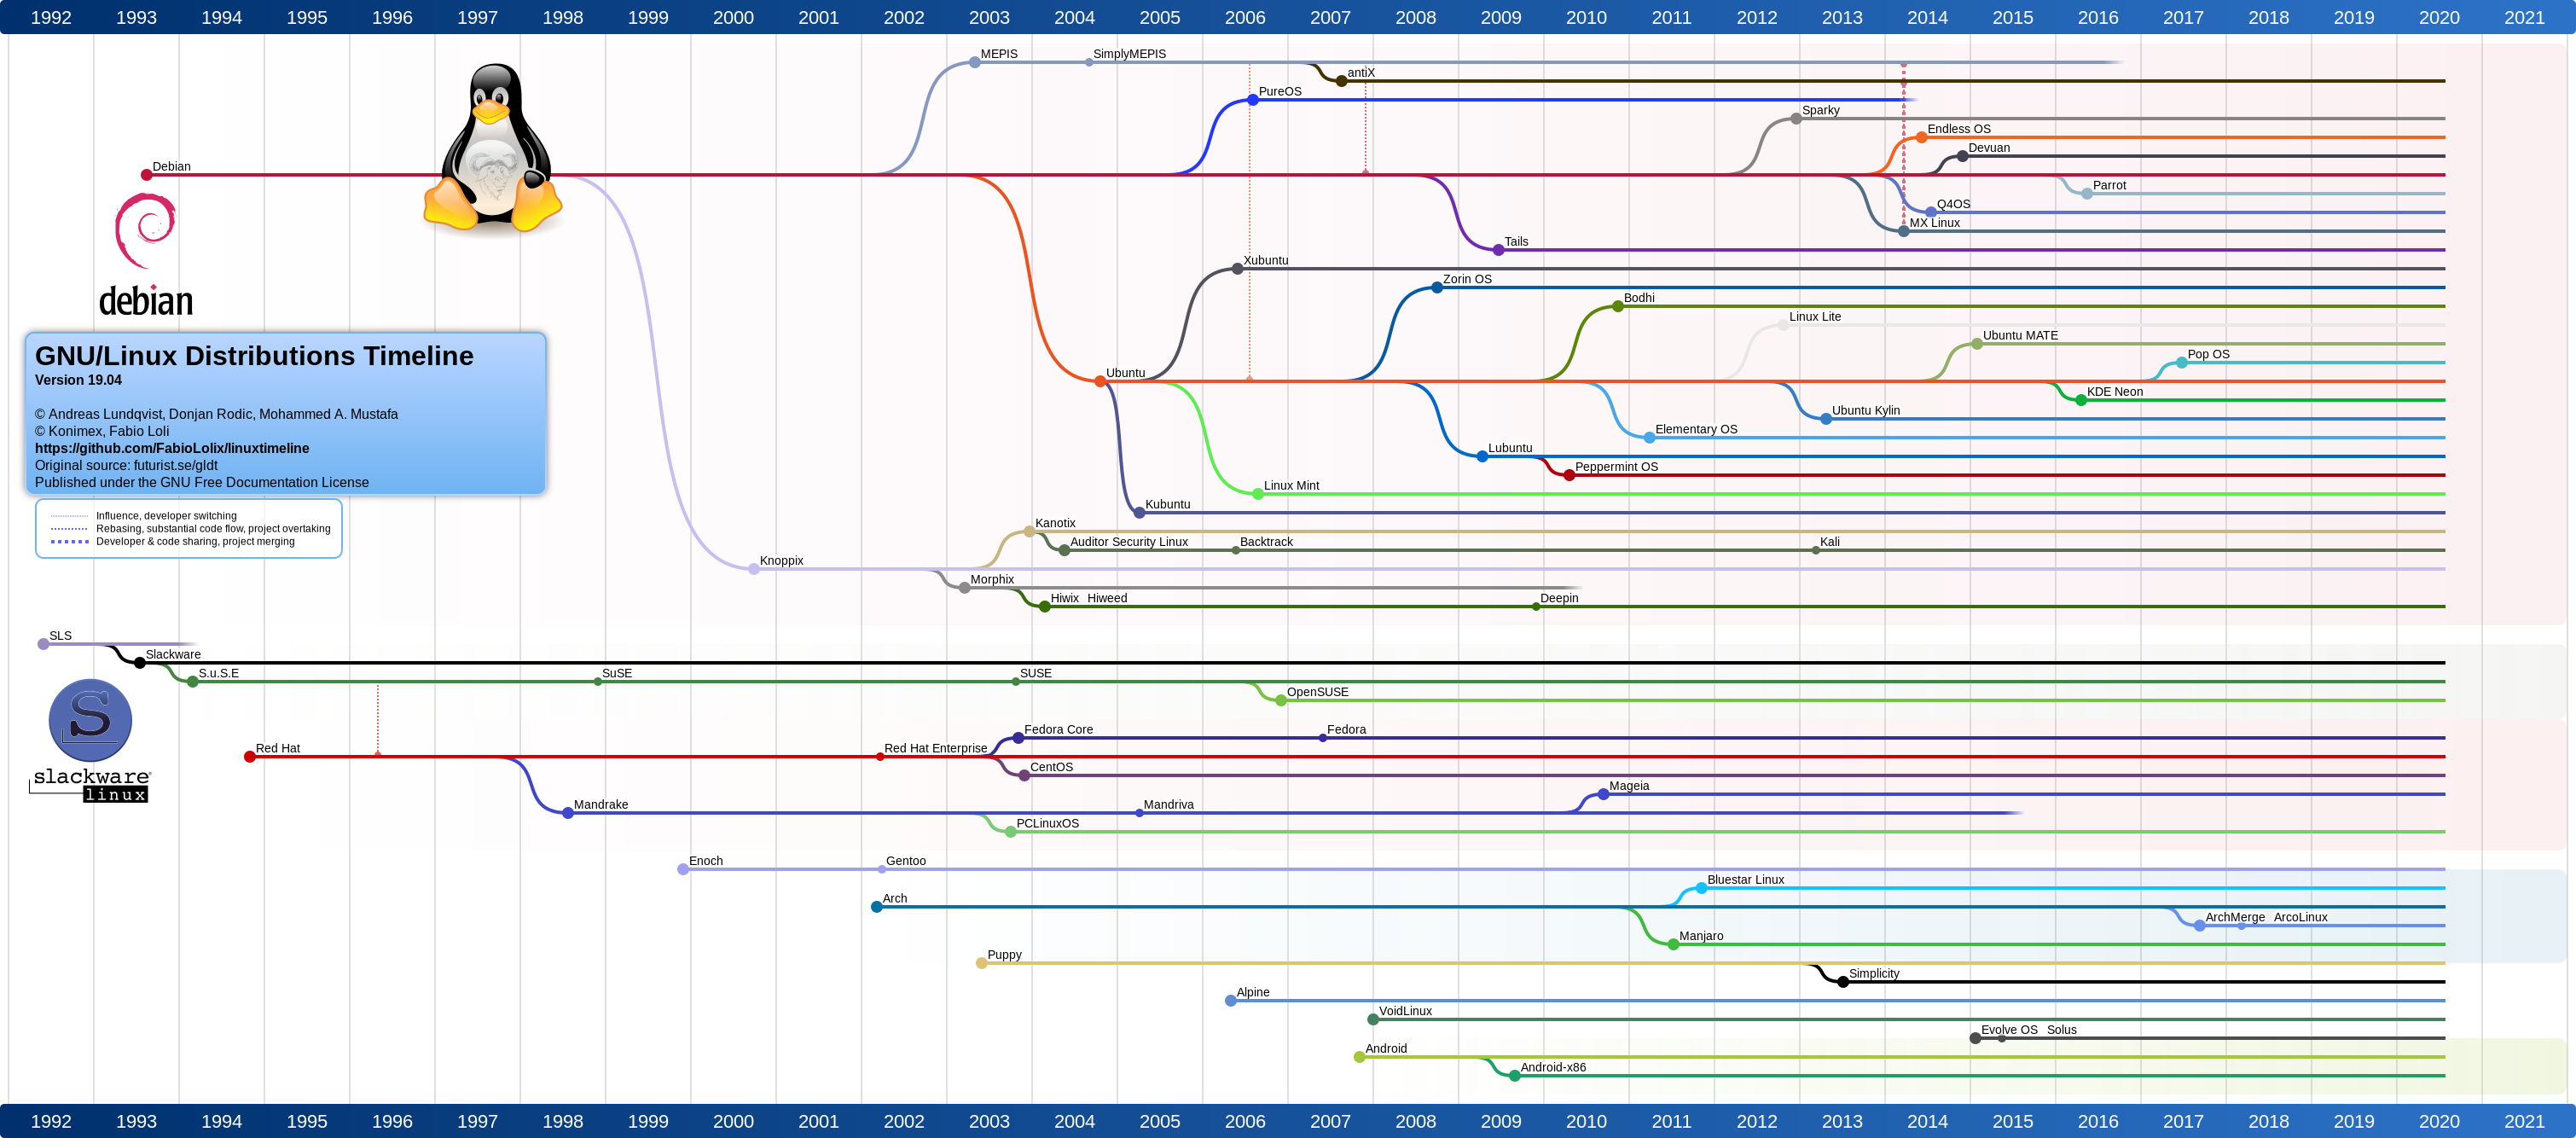
\includegraphics[scale=0.18]{images/aygzaivcbmd51.png}
\end{frame}

\begin{frame}{Le distribuzioni GNU/Linux oggi}
Possiamo suddividere le distribuzioni in GNU/Linux in famiglie:
\begin{itemize}
    \item Debian(Ubuntu, MX Linux, Kali Linux)
    \item Ubuntu(Linux Mint, Elementary OS, Zorin OS)
    \item Arch Linux(Manjaro, EndeavourOS)
    \item Fedora
    \item Gentoo
    \item ...
\end{itemize}

\end{frame}

%------------------------------------------------
